\section{First prototype} \label{ch:first_prototype}

To create a first prototype capable of detecting hand-drawn mechanism, the capabilities necessary are have to be considered first.
The application has to be able to detect and to localize \name{nodes} and to detect \name{constraints}, which are connecting pairs of \name{nodes}.
Subsequently the gathered information has to be transformed into a usable format for further processing.

At first the detection and localization of \name{nodes} is examined.

\subsection{The Fully Convolutional Network}\label{ch:fcn}

The topic of a previous work was the recognition of hand-drawn mechanical symbols \cite{Lawrence2020}.
Building on this, the trained model is improved to provide not only the class, but the location of the classification in an image of arbitrary size.

The respective model can be loaded using \name{Keras'}, % TODO citation should be in the introduction.
\code{model.load\_model} and by issuing the \code{summary} method we get listing~\ref{lst:srp_model}.

\begin{lstlisting}[caption={Summary of Symbol Classifier}, label={lst:srp_model}]
_________________________________________________________________
Layer (type)                 Output Shape              Param #
=================================================================
conv2d (Conv2D)              (None, 32, 32, 16)        272
_________________________________________________________________
max_pooling2d (MaxPooling2D) (None, 16, 16, 16)        0
_________________________________________________________________
conv2d_1 (Conv2D)            (None, 16, 16, 32)        8224
_________________________________________________________________
max_pooling2d_1 (MaxPooling2 (None, 8, 8, 32)          0
_________________________________________________________________
flatten (Flatten)            (None, 2048)              0
_________________________________________________________________
dense (Dense)                (None, 3)                 6147
=================================================================
Total params: 14,643
Trainable params: 14,643
Non-trainable params: 0
_________________________________________________________________
\end{lstlisting}

One way to localize images in a bigger image is to scan each sector of an image and predicting the generated crops.
Using a 360x360 sized image, a stride of one in each direction, the number of images which are used in the prediction process are 108.241 images\footnote{$h + 1 - 32 * w + 1 - 32$, where $h$ and $w$ are the height and width of the input image and the size of the kernel used to predict is 32}.
A Jupyter notebook to test the performance on this can be found at \url{https://aka.klawr.de/sep#1}. % TODO Set this URL.

To test this amount of images is often not necessary and can be reduced by increasing the stride of the respective scanning process.
This would reduce the accuracy of the localization, but would increase the speed.

Another approach is to use the properties of convolutional layer to restructure the model and thereby making the whole procedure much more efficient.

By transforming a model into a Fully Convolutional Network (FCN) all dense layers are replaced by convolutional layers, and the input layer is also a two dimensional layer but allows for an input image of arbitrary size.
Because the input of the original model is only defined by the kernel size, it is agnostic to the size of a previous layer.
Listing \ref{lst:to_fcn} transforms the \code{old\_model} by appending an \code{tf.keras.Input} layer without any specified size and replacing the output layer by a \code{tf.keras.Conv2D} layer\footnote{And thus removing the \code{tf.keras.flatten} layer.}

\begin{lstlisting}[caption={Transformation into a FCN}, label=lst:to_fcn]
inputs = tf.keras.Input(shape=(None, None, 1))

hidden = old_model.layers[0](inputs)

for layer in old_model.layers[1:4]:
    hidden = layer(hidden)

# Get the input dimensions of the flattened layer:
f_dim = old_model.layers[4].input_shape
# And use it to convert the next dense layer:
dense = old_model.layers[5]
out_dim = dense.get_weights()[1].shape[0]
W, b = dense.get_weights()
new_W = W.reshape((f_dim[1], f_dim[2], f_dim[3], out_dim))
outputs = tf.keras.layers.Conv2D(out_dim,
                           (f_dim[1], f_dim[2]),
                           name = dense.name,
                           strides = (1, 1),
                           activation = dense.activation,
                           padding = 'valid',
                           weights = [new_W, b])(hidden)

model = tf.keras.Model(inputs = inputs, outputs = outputs)

model.summary()
\end{lstlisting}

An example for the usage of this code can be found at \url{https://aka.klawr.de/sep#2} % TODO
, where the intricate differences between both approaches are discussed.

The FCN approach is roughly ten times faster than taking crops and predicting them individually. 
This \code{model.summary} results in the following output:

\begin{lstlisting}
Model: "model"
_________________________________________________________________
Layer (type)                 Output Shape              Param #   
=================================================================
input_1 (InputLayer)         [(None, None, None, 1)]   0         
_________________________________________________________________
conv2d (Conv2D)              multiple                  272       
_________________________________________________________________
max_pooling2d (MaxPooling2D) multiple                  0         
_________________________________________________________________
conv2d_1 (Conv2D)            multiple                  8224      
_________________________________________________________________
max_pooling2d_1 (MaxPooling2 multiple                  0         
_________________________________________________________________
dense (Conv2D)               (None, None, None, 3)     6147      
=================================================================
Total params: 14,643
Trainable params: 14,643
Non-trainable params: 0
_________________________________________________________________
\end{lstlisting}

Granted this model is satisfactory for the moment, the problem of detecting constraints can be addressed.

\subsection{Constraint detection}

There was already a model providing the capability of detecting symbols, to prior work.
To create a model for detecting constraints the same procedure has to be followed, which means that training data has to be generated first.

It is planned to support two different types of constraints, which indicate whether two nodes are either able to rotate around one another or to be able to move in a translational fashion.
Beside different types of constraints data for three different ranges are generated for a better selection of constraint data when two nodes are to be connected.

Data generation for constraints is similar to data generation in \cite{Lawrence2020}.
The drawing canvas has a width of fifty and the range can vary between 150-249, 250-349 or 350-449; depending on the selected range.

\begin{figure}
    \centering
    \begin{subfigure}[b]{0.45\textwidth}
        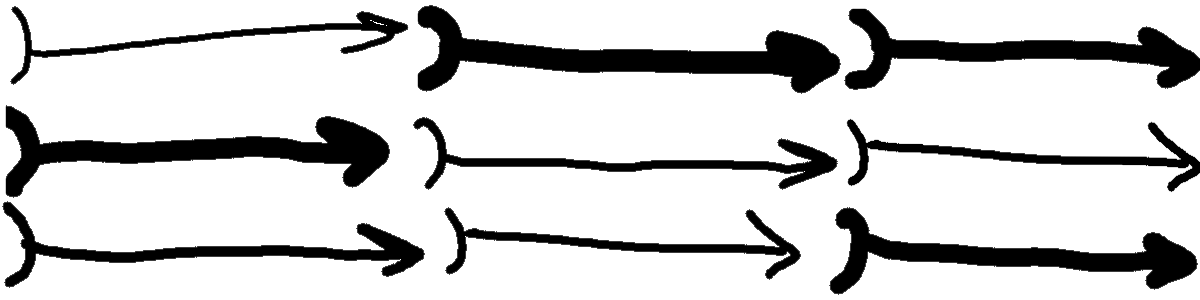
\includegraphics[width=\textwidth]{images/rs.png}
        \caption{Rotational Constraints}
        \label{fig:rotational_constraints}
    \end{subfigure}
    \begin{subfigure}[b]{0.45\textwidth}
        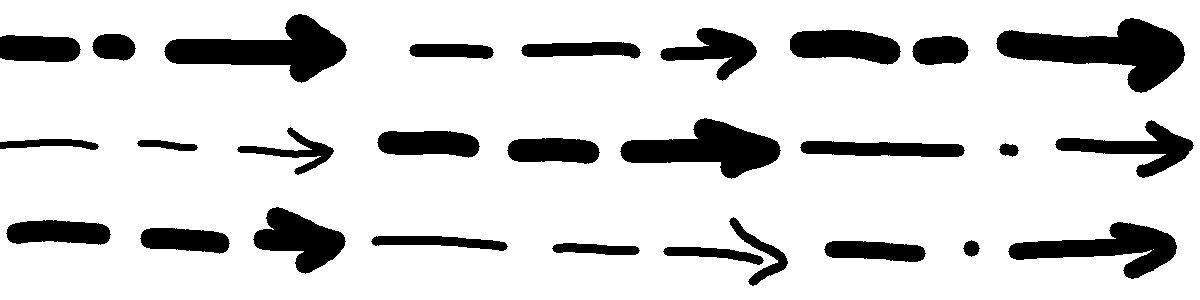
\includegraphics[width=\textwidth]{images/ts.png}
        \caption{Translational Constraints}
        \label{fig:translational_constraints}
    \end{subfigure}
    \caption{Some examples of the data created with the described method. Only these two classes were created for the first tests. The images are created horizontally, so their initial angle can be assumed to be zero to keep record when labeling the data dynamically. }
    \label{fig:generated_data_samples}
\end{figure}

\subsubsection{Preparing nodes on images}

Since constraints can occur at all possible angles, the data must be generated in such a way that it resembles the reality the most.
Because of this, multiple steps have to be taken to generate comprehensible data.

Metadata generated during the generation process is saved into a format which is readable by \name{pandas}. % TODO citation needed
\name{pandas} is a open source data analysis and manipulation tool which helps to work and to visualize data.

In the first step 100.000 images are generated.
Each image begins with a black background of size 360x360.
Between 3 and 10 nodes are randomly placed on the image\footnote{In an intermediate step the node data from previous work is modified to consist of white symbols on black background, instead of random grayscale images.}.
Each node has to have a minimum distance of 60 to every other node in the image.
Examples for the resulting images are shown in figure \ref{fig:constraint_data_step1}.
The respective notebook containing the code for this process can be viewed at \url{https://aka.klawr.de/sep\#3}.

\begin{figure}
    \centering
    \label{fig:constraint_data_step1}
    \begin{subfigure}[b]{0.19\textwidth}
        \fbox{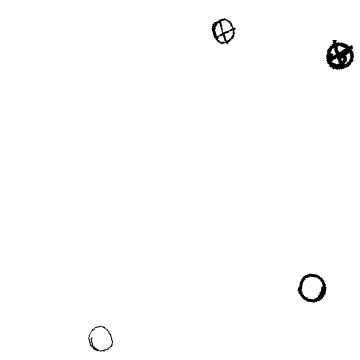
\includegraphics[width=\textwidth]{images/1_0.png}}
    \end{subfigure}
    \begin{subfigure}[b]{0.19\textwidth}
        \fbox{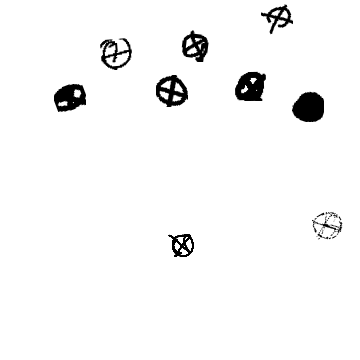
\includegraphics[width=\textwidth]{images/1_1.png}}
    \end{subfigure}
    \begin{subfigure}[b]{0.19\textwidth}
        \fbox{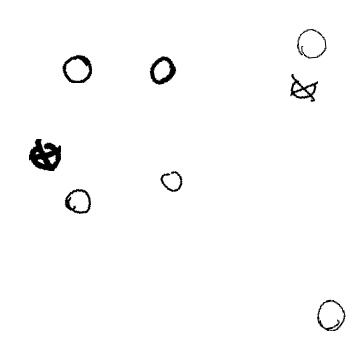
\includegraphics[width=\textwidth]{images/1_2.png}}
    \end{subfigure}
    \begin{subfigure}[b]{0.19\textwidth}
        \fbox{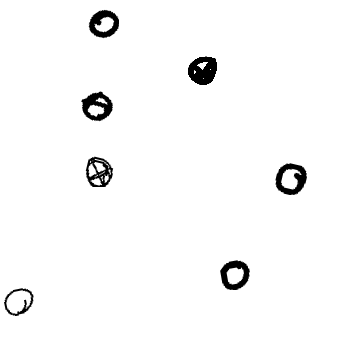
\includegraphics[width=\textwidth]{images/1_3.png}}
    \end{subfigure}
    \begin{subfigure}[b]{0.19\textwidth}
        \fbox{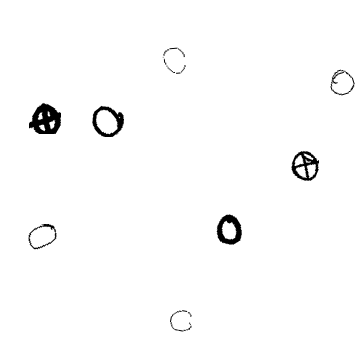
\includegraphics[width=\textwidth]{images/1_4.png}}
    \end{subfigure}
    \caption{Some examples of the data created with the described method. Please note that the colors of these samples are inverted. }
\end{figure}

% TODO add more text... to many images for little text

\subsubsection{Connecting nodes using constraints}

The next step is to randomly connect pairs of nodes inside of the image.
For this the prepared constraints are used, whereas the number of constraints should be random, too.

On an image with $n$ nodes the number of possible connections is $\frac{n \times (n-1)}{2}$.
As a reasonable heuristic to keep the number of constraints in check $s = 1 - \frac{2}{n-1}$ is used; where $s$ is the chance of the connection being skipped and $n$ is the number of nodes.

Table \ref{tab:relation_nodes_constraints} describes the expected number of constraints per image.
This approach tries to generate as much constraints as there are nodes in the image.
The difference of the expected number of constraints and the mean of constraints per number of nodes in table \ref{tab:relation_nodes_constraints} occurs most likely due to constraints shorter than 50 or longer than 350 being skipped, too.
The mean of the number of constraints in relation to the number of nodes is calculated by issuing \code{[df[df.nodes.str.len() == i].constraints.str.len().mean() for i in range(3,10)]}, where \code{df} is the respective \code{pandas.DataFrame}.

\begin{table}
\caption{Relation of number of nodes to the resulting number of constraints.}
\label{tab:relation_nodes_constraints}
\begin{tabular}{lrrrrrrr}
    \toprule
    Number of nodes: & $3$ & $4$ & $5$ & $6$ & $7$ & $8$ & $9$ \\
    \midrule
    Possible connections: & $3$ & $6$ & $10$ & $15$ & $21$ & $28$ & $36$ \\
    \midrule
    Chance to skip node pair: & $0$ & $\frac{1}{3}$ & $\frac{1}{2}$ & $\frac{3}{5}$ & $\frac{2}{3}$ & $\frac{5}{7}$ & $\frac{3}{4}$ \\
    \midrule
    Expected number of constraints: & $3$ & $4$ & $5$ & $6$ & $7$ & $8$ & $9$ \\
    \midrule
    Mean of constraints in the dataset: & $2.62$ & $3.48$ & $4.35$ & $5.21$ & $6.10$ & $6.91$ & $7.78$ \\
    \bottomrule
\end{tabular}
\end{table}

The images which are generated in this step are shown in figure \ref{fig:constraint_data_step2}\footnote{In the initial dataset for constraints 3 different types were made for different length-intervals. After initial testing the shorter constraints did not meet the visual expectations. Thus these images are generated with images from a range of 350-449 only.}.

\begin{figure}
    \centering
    \label{fig:constraint_data_step2}
    \begin{subfigure}[b]{0.19\textwidth}
        \fbox{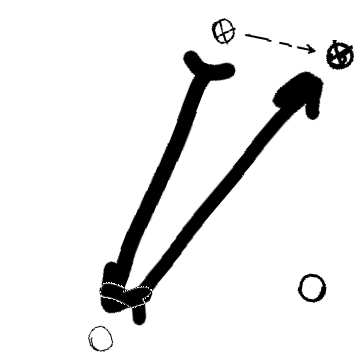
\includegraphics[width=\textwidth]{images/2_0.png}}
    \end{subfigure}
    \begin{subfigure}[b]{0.19\textwidth}
        \fbox{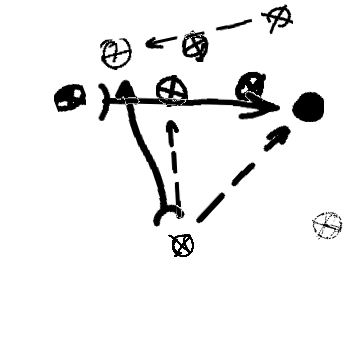
\includegraphics[width=\textwidth]{images/2_1.png}}
    \end{subfigure}
    \begin{subfigure}[b]{0.19\textwidth}
        \fbox{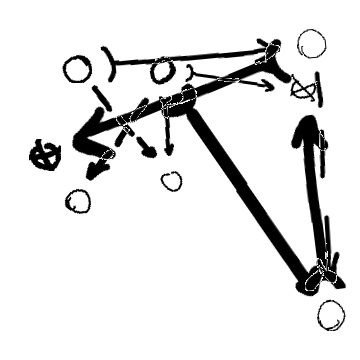
\includegraphics[width=\textwidth]{images/2_2.png}}
    \end{subfigure}
    \begin{subfigure}[b]{0.19\textwidth}
        \fbox{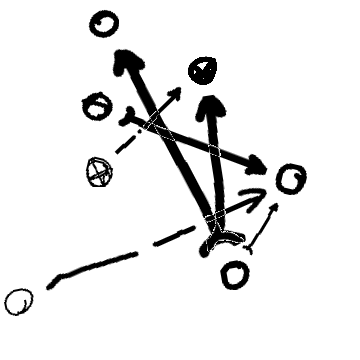
\includegraphics[width=\textwidth]{images/2_3.png}}
    \end{subfigure}
    \begin{subfigure}[b]{0.19\textwidth}
        \fbox{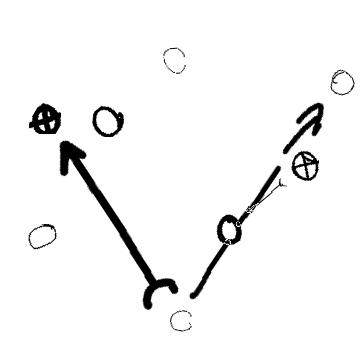
\includegraphics[width=\textwidth]{images/2_4.png}}
    \end{subfigure}
    \caption{Samples of images generated by connecting randomly selected pairs of nodes using the prepared constraint data. Please note that the colors of these samples are inverted.}
\end{figure}

\subsubsection{Cropping images to get the training data}

At last these images are cropped.
By cropping and reshaping the models the images can be fed into the training process of a Keras model.
The notebook doing this operation can be viewed at \url{https://aka.klawr.de/sep\#4}.
As the number of possible connections is $34 = \frac{\sum_{i=3}^{9}i(i-1)}{(10-3)}$, the expected number of generated crop-images is 3.400.000.
It is also important to check for reversed constraints between node pairs to classify them as a non connection, to be able to correctly predict the direction of the constraint, too.
As 100.000 images are already a good size to work with, another measure was taken to keep the number of expected crops in check.
For this crops are only kept $\frac{1}{m(m-1)}$ of the time, which is about each 30th time in this case.

The resulting dataset contains 119.189 images, which are subsequently transformed into a \name{tensorflow record}.

% TODO image of the crops here...

With the data prepared the next step is to train the constraint detecting model.

\subsubsection{Training of the constraint detection model}

In this first prototype the design of the constraint detection model is a copy of the results of the previous trained symbol detector.
The input size is adapted to fit for the crops, which have a size of 96 by 96 instead of the 32 by 32 images used for the symbol detector.
The model is created using the functional API of Keras, which has no functional implications, but is just another way of defining models.

The output of \code{model.summary()} is:
\begin{lstlisting}
Model: "model"
_________________________________________________________________
Layer (type)                 Output Shape              Param #   
=================================================================
input_1 (InputLayer)         [(None, 96, 96, 1)]       0         
_________________________________________________________________
conv2d (Conv2D)              (None, 96, 96, 16)        272       
_________________________________________________________________
max_pooling2d (MaxPooling2D) (None, 48, 48, 16)        0         
_________________________________________________________________
conv2d_1 (Conv2D)            (None, 48, 48, 32)        8224      
_________________________________________________________________
max_pooling2d_1 (MaxPooling2 (None, 24, 24, 32)        0         
_________________________________________________________________
flatten (Flatten)            (None, 18432)             0         
_________________________________________________________________
dense (Dense)                (None, 3)                 55299     
=================================================================
Total params: 63,795
Trainable params: 63,795
Non-trainable params: 0
_________________________________________________________________    
\end{lstlisting}

The training is done by decoding the record which was created in earlier steps
and then splitting the data into 80.000 images for training, 20.000 images for validation and the remaining 19.189 images are used for testing the model.

The training is then initiated by using the \code{model.fit} method, passing the data as argument.
\name{TensorBoard} % TODO citation needed
is used to log the accuracy and the loss of the model during training. The respective graphs can be seen in figure \cite{fig:crop_detector_tensorboard}.

\begin{figure}[]
    \centering
    \begin{subfigure}[b]{0.45\textwidth}
        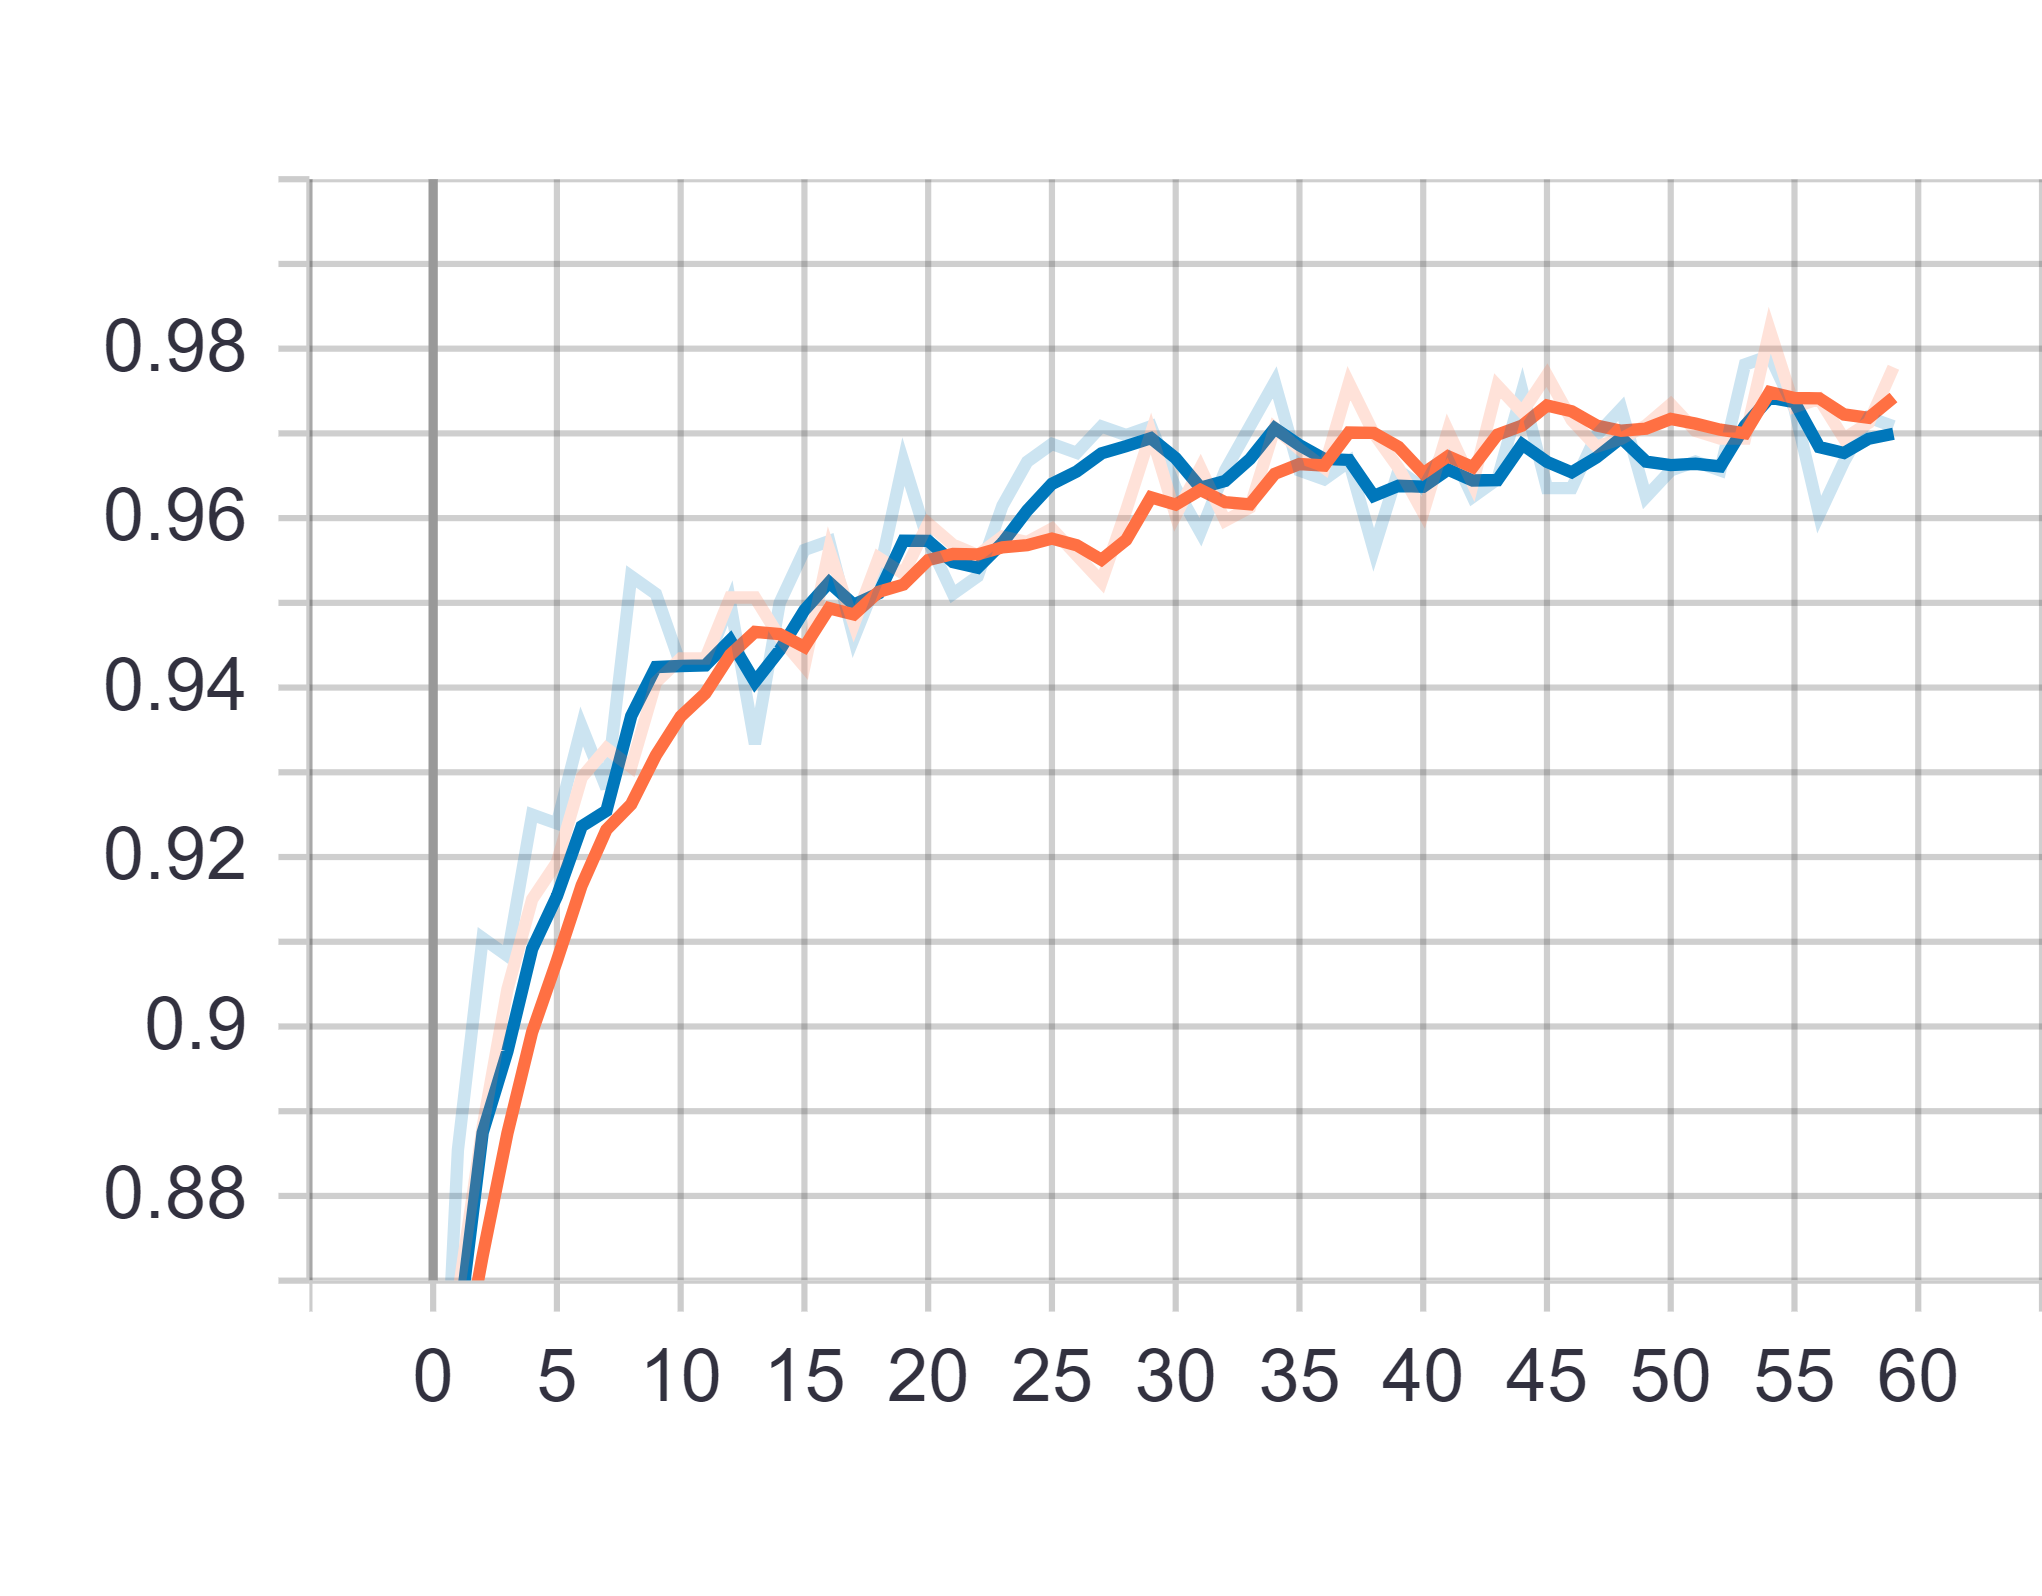
\includegraphics[width=\textwidth]{images/crop_detector_epoch_acc.png}
    \end{subfigure}
    \begin{subfigure}[b]{0.45\textwidth}
        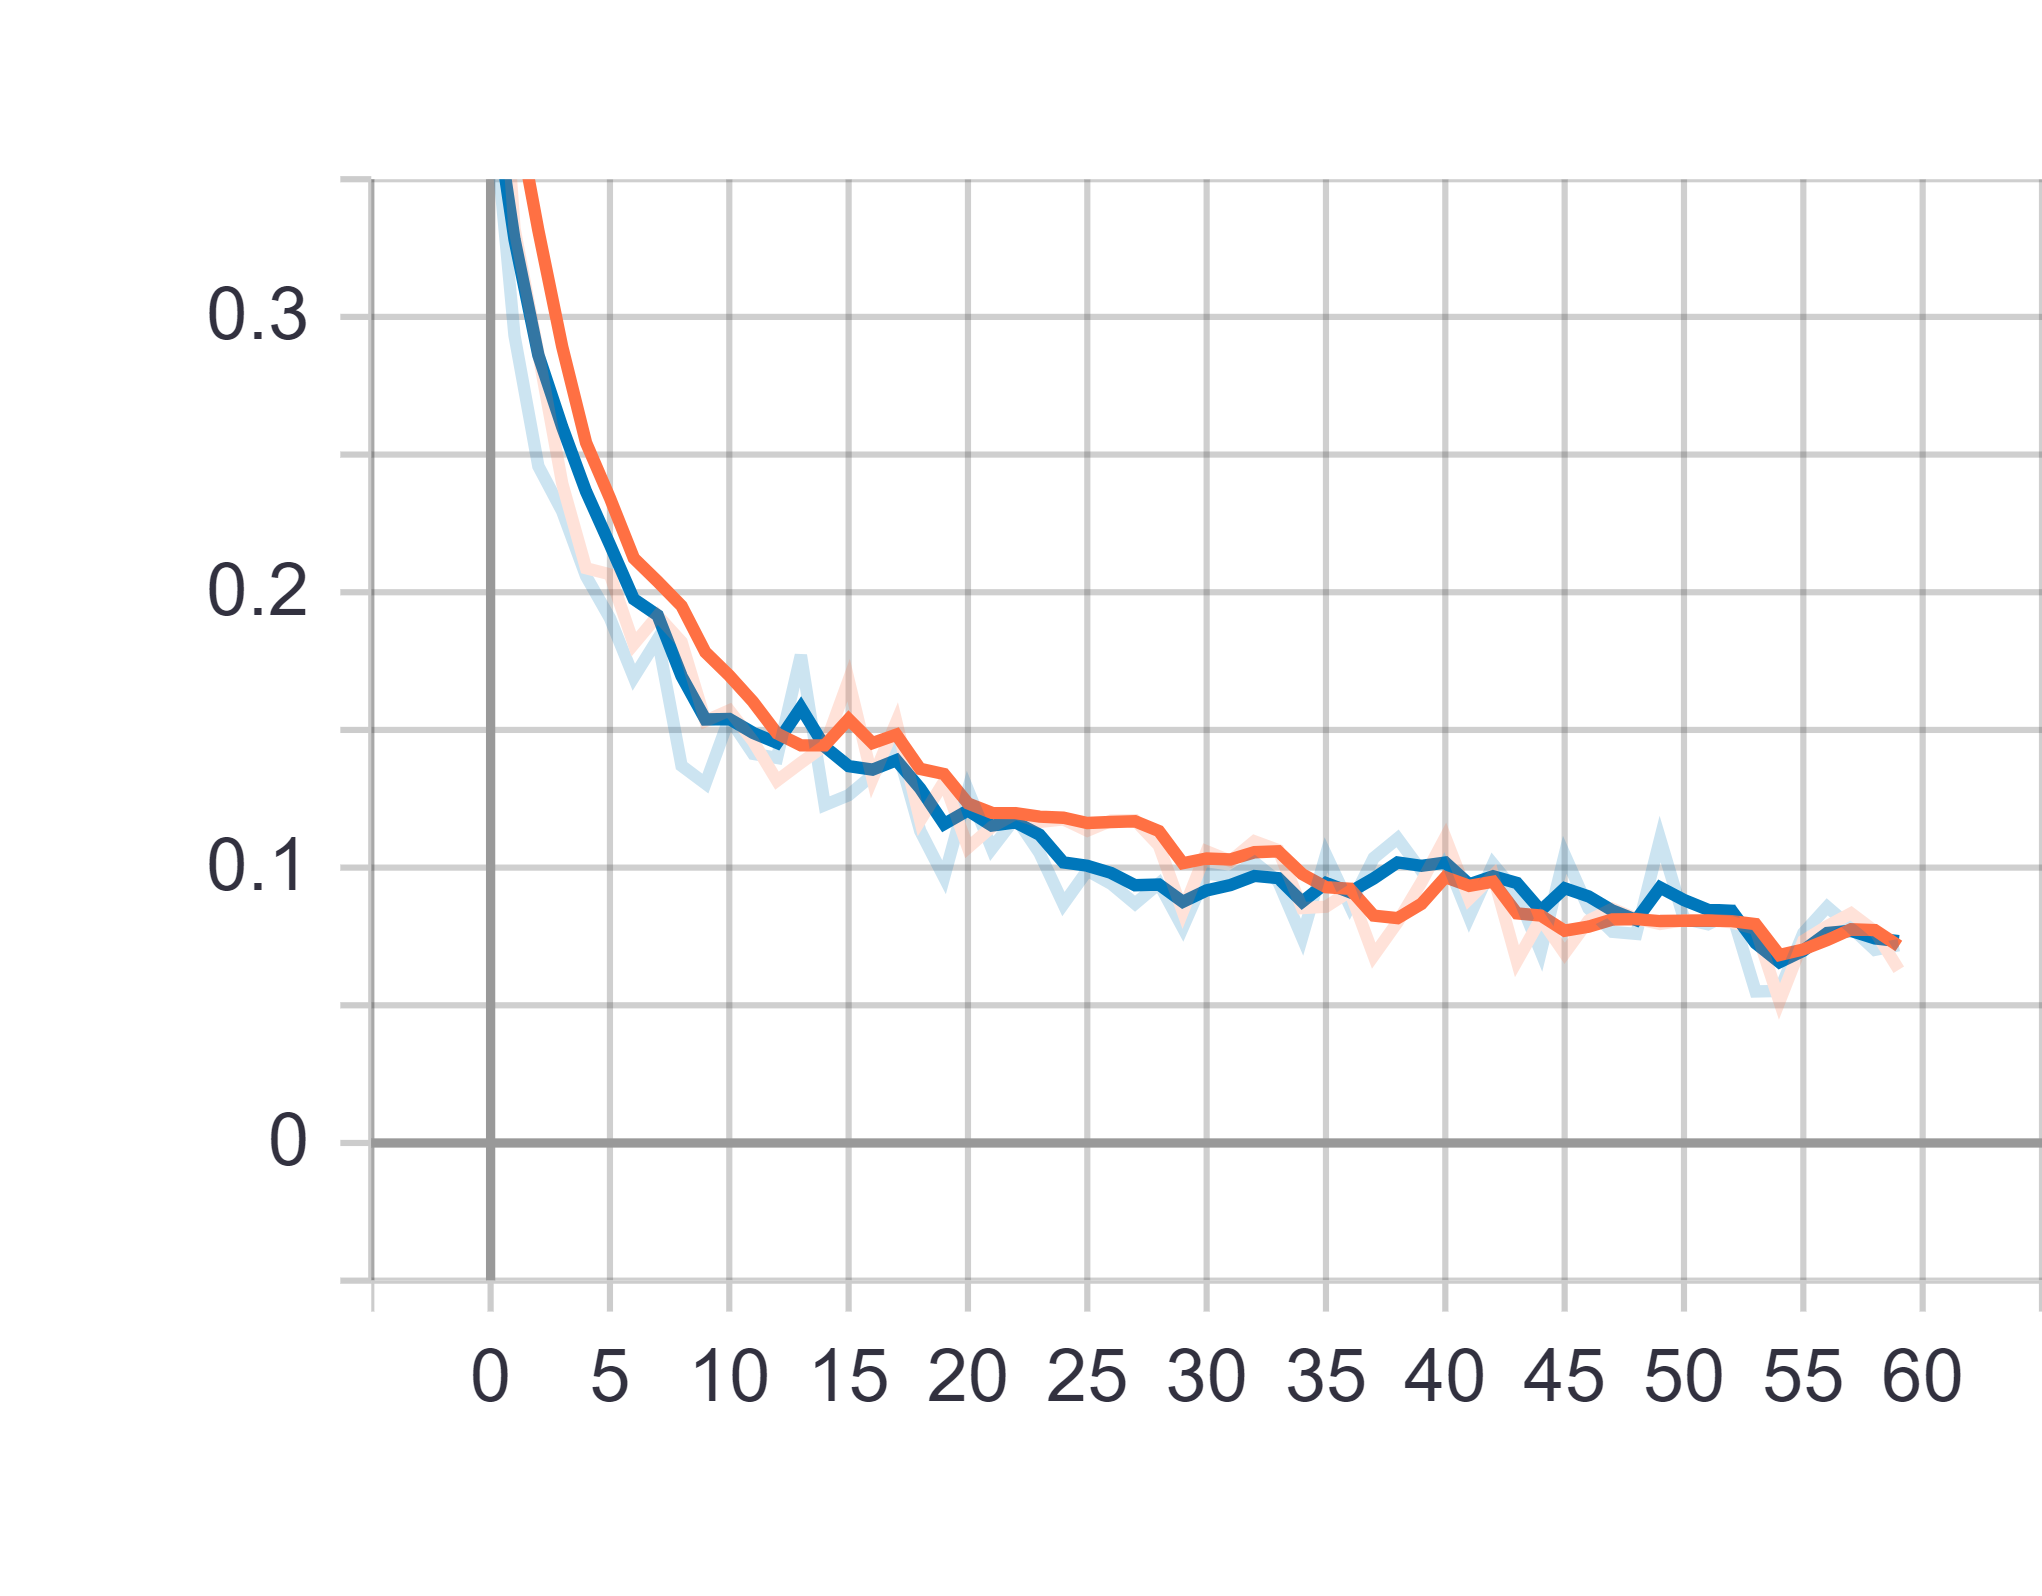
\includegraphics[width=\textwidth]{images/crop_detector_epoch_loss.png}
    \end{subfigure}
    \caption{The training accuracy and loss of the crop detector. These graphs were created using TensorBoard, which is used as callback during training.}
    \label{fig:crop_detector_tensorboard}
\end{figure}

\subsubsection{Combining node and constraint detection}

To be able to predict constraints in production the generation of crops has to be implemented as a intermediate step between node and constraint detection.
The images must be cropped according to the generation of the training data, which means the coordinates of the nodes have to be detected first, and the area between them is resized to 96 by 96 images.
Previously the nodes are placed on the image using (randomly) given coordinates.
This process is now revered, getting the coordinates using the Fully Connected Network on the training data and processing the data.

The constraint detection relies heavily on the performance of the node detection, because nodes which are not detected are not taken into account when creating the data for the constraint detector.

Falsely predicted nodes are most likely not going to result in a pair of nodes connected by constraints, since the resulting crop would most likely not look like a constraint, but they are slowing the process down significantly, since the number of crops grows exponentially to the number of nodes.

A pipeline of this process can be reviewed at \url{https://aka.klawr.de\#5}.

\begin{figure}
    \centering
    \label{fig:constraint_data_step1}
    \begin{subfigure}[b]{0.19\textwidth}
        \fbox{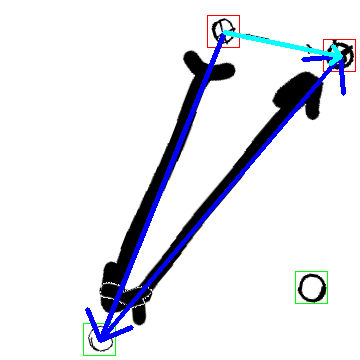
\includegraphics[width=\textwidth]{images/225_0rc.png}}
    \end{subfigure}
    \begin{subfigure}[b]{0.19\textwidth}
        \fbox{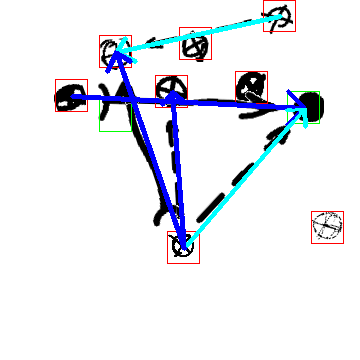
\includegraphics[width=\textwidth]{images/225_1rc.png}}
    \end{subfigure}
    \begin{subfigure}[b]{0.19\textwidth}
        \fbox{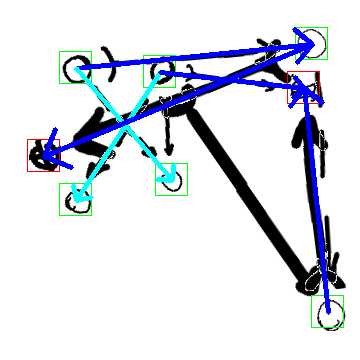
\includegraphics[width=\textwidth]{images/225_2rc.png}}
    \end{subfigure}
    \begin{subfigure}[b]{0.19\textwidth}
        \fbox{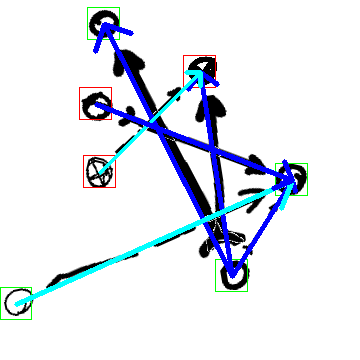
\includegraphics[width=\textwidth]{images/225_3rc.png}}
    \end{subfigure}
    \begin{subfigure}[b]{0.19\textwidth}
        \fbox{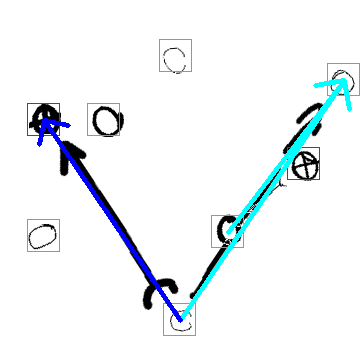
\includegraphics[width=\textwidth]{images/225_4rc.png}}
    \end{subfigure}
    \caption{The second step of the data generation processed created images with nodes and constraints that resemble nodes and constraints placed randomly into a canvas. These predictions are made on the images from figure \ref{fig:constraint_data_step2}. There is only one falsely predicted node in the second image from the left. The constraints are way less accurate, which is not surprising considering the composition of these images.}
\end{figure}
